% To enable the camera-ready format, use the following line
%\documentclass{gtac}

% To enable the double-blind submission format for the review process, use the following line
\documentclass[blind]{gtac}

\usepackage{cite}

% This is the watermark text. 
\SetWatermarkText{
  \shortstack{
        AMD Internal Use Only  \\[1em]  GTAC 2024 
  }
}
\SetWatermarkScale{0.3}
\SetWatermarkAngle{30}
\SetWatermarkColor{gray!20}


\title{FIXME: title \subtitle{Submitted Anonymously for Double-Blind Review}}


\author{Malcolm Roberts \\
AIG Software Development \\
malcolm.roberts@amd.com}


\begin{document}

\maketitle % Create the title section
\vspace*{-1.2in} % Adjust this value to reduce the space


% Used to fix the header. 
\pagestyle{fancy}
\fancyhf{} % clear all header and footer fields
\cfoot{\thepage} % put the page number in the center of the footer
\renewcommand{\headrulewidth}{0pt} % Remove the horizontal line from header
%\chead{\textcolor{gray}{Proceedings of the 2024 AMD Global Technical Authors Conference – AMD Internal Use Only}}
\chead{{\sffamily\textcolor{red}{\fontsize{10}{12}\selectfont\textbf{DO NOT FORWARD – FOR GTAC’24 REVIEW COMMITTEE ONLY}}}}

\thispagestyle{fancy}
\begin{abstract}
The performance of bandwidth-limited algorithms strongly depends on compute memory hierarchy.  In
this article, we propose a model for FFT performance on ROCm GPUs as a function of shared memory
(LDS) size and performance.
\end{abstract}

\keywords{FFT, GPU, LDS, ROCm}

\section{Introduction}

the fast Fourier transforms (FFT) is considered one of the most important algorithms of the modern
era~\cite{strang1994wavelets} and has a variety of important uses from digital signal
processing~\cite{sorensen1990efficient}, to computational fluid
mechanics~\cite{chatterjee2018scaling}, to machine learning~\cite{mathieu2013fast}, and many others.

TODO: talk about N log N, so bandwidth-limited.  Also, all-to-all.  Thus, need LDS.

TODO: cache-oblivious algorithms~\cite{frigo1999cache}

TODO: L1DCC~\cite{bailey1990ffts}

FIXME

\subsection{Comments on Formatting}

ref: \begin{verbatim}bailey-ffts_external_memory-1989.pdf\end{verbatim}

Do not change the format of the main body of text, the headings, margin sizes, gutter width, title
and author block, bibliography, etc.  This includes modifications to the font, font size, line
spacing, kerning, etc. \ul{Abusing the \LaTeX~formatting to circumvent page/content limits can
  result in an administrative rejection without further review.} This is a sample
footnote. \footnote{A sample footnote.}

Figures and tables should be accompanied by a numbered label and caption as shown in the Figure
\ref{fig:1} and Figure \ref{fig:2}. Note that we used 'h' position for Figure \ref{fig:1} and 't'
for Figure \ref{fig:2}.


\begin{figure}[h] % 'h' means "here"
    \centering
    
\includegraphics[width=0.4\textwidth]{fig1}
    \caption{Insert figures using includegraphics.}
    \label{fig:1}
\end{figure}

\begin{figure}[h] % 't' means "here"
    \centering
    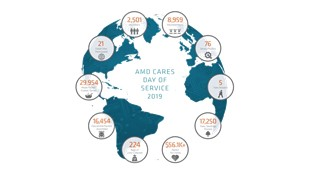
\includegraphics[width=0.4\textwidth]{fig2}
    \caption{Statistics related to last year's AMD Cares Day of Service.}
    \label{fig:2}
\end{figure}

\subsection{Heading Level 2}
This is an example of heading level 2.

\subsubsection{Heading Level 3}
This is an example of heading level 3.

\section{Another Section (dummy text)}

\lipsum[1-10] % generates dummy text


\section{Conclusions}
The conclusions section should state key conclusions and insights.  While perhaps not entirely
“conclusive”, this is also a good place to discuss any limitations of the work covered in this paper
(e.g., “we focused on the DL1 cache but have not yet extended the analysis to the L2”), speculations
for future directions (e.g., “the results were promising for machine learning workloads, and due to
our matrix-oriented optimizations we expect our technique to have some potential for scientific
computing”), and any commentary on potential, planned, or actual impact on AMD (e.g., hardware,
software, tools, methodologies, roadmap).  The last part is useful to provide the reviewers with
additional context on the broader value of the work.  We recommend simply cut-and-pasting or
re-summarizing the abstract as that does not really add any value to the paper.

\begingroup
\let\itshape\upshape
\bibliographystyle{abbrv}
\bibliography{refs}
\endgroup

\section*{\st{Acknowledgments}}
Do \ul{not} include acknowledgments in this blind-review version of the paper, as acknowledgments
may provide unintended hints that “deblind” your anonymity. If your paper is accepted to GTAC, the
final published version can/should include the appropriate acknowledgments.

\end{document}
